\documentclass{beamer}

\usepackage{amsmath}
\usepackage{amssymb}
\usepackage{mathtools}
%\usepackage{float}
%\usepackage[pdftex]{graphicx}
\usepackage{ngerman}
%\usepackage[T1]{fontnc}
\usepackage[utf8]{inputenc}
%\usepackage{enumerate}
%\usepackage{ifpdf}

\usetheme{Warsaw}

\title{Elektronikpraktikum SS14, Auswertung: Versuchstag 1}
\author{Gruppe 1 \\ Patrick Heuer \\ Benjamin Lotter}
\date{}

\begin{document}
\frame{\titlepage}
%\tableofcontents

\begin{frame}
    \frametitle{Aufgabe 1a}
    \framesubtitle{Schaltplan}
    Hier kommen die Schaltpläne hin
\end{frame}
\begin{frame}
    \frametitle{Aufgabe 1a}
    \framesubtitle{Messreihen}
    Hier kommt die Messreihe hin.
\end{frame}
\begin{frame}
    \frametitle{Aufgabe 1a}
    \framesubtitle{Beobachtungen}
    Hörbares klicken im DMM bei Übergängen 
    \begin{align*}
        \text{Aufwärts:}\quad&
        220mV-240mV\qquad
        280mV-300mV\\
        \text{Abwärts:}\quad&
        60mV-40mV\qquad
        4mV-3mV
    \end{align*}
    \rightarrow 
\end{frame}
\begin{frame}
    \frametitle{Aufgabe 1a}
    \framesubtitle{benis}
    sadf
\end{frame}
%\begin{frame}
%    \frametitle{Aufgabe 1a}
%    \framesubtitle{}
%    \pause
%\end{frame}
%\begin{frame}
%    \frametitle{Aufgabe 1a}
%    \framesubtitle{}
%    \pause
%\end{frame}
%\begin{frame}
%    \frametitle{Aufgabe 1a}
%    \framesubtitle{}
%    \pause
%\end{frame}
%\begin{frame}
%    \frametitle{Aufgabe 1a}
%    \framesubtitle{}
%    \pause
%\end{frame}
%\begin{frame}
%    \frametitle{Aufgabe 1a}
%    \framesubtitle{}
%    \pause
%\end{frame}
%\begin{frame}
%    \frametitle{Aufgabe 1a}
%    \framesubtitle{}
%    \pause
%\end{frame}
%\begin{frame}
%    \frametitle{Aufgabe 1a}
%    \framesubtitle{}
%    \pause
%\end{frame}
%\begin{frame}
%    \frametitle{Aufgabe 1a}
%    \framesubtitle{}
%    \pause
%\end{frame}
%\begin{frame}
%    \frametitle{Aufgabe 1a}
%    \framesubtitle{}
%    \pause
%\end{frame}
%\begin{frame}
%    \frametitle{Aufgabe 1a}
%    \framesubtitle{}
%    \pause
%\end{frame}
%\begin{frame}
%    \frametitle{Aufgabe 1a}
%    \framesubtitle{}
%    \pause
%\end{frame}
%\begin{frame}
%    \frametitle{Aufgabe 1a}
%    \framesubtitle{}
%    \pause
%\end{frame}
%\begin{frame}
%    \frametitle{Aufgabe 1a}
%    \framesubtitle{}
%    \pause
%\end{frame}
%\begin{frame}
%    \frametitle{Aufgabe 1a}
%    \framesubtitle{}
%    \pause
%\end{frame}
%\begin{frame}
%    \frametitle{Aufgabe 1a}
%    \framesubtitle{}
%    \pause
%\end{frame}
%\begin{frame}
%    \frametitle{Aufgabe 1a}
%    \framesubtitle{}
%    \pause
%\end{frame}
%\begin{frame}
%    \frametitle{Aufgabe 1a}
%    \framesubtitle{}
%    \pause
%\end{frame}
%\begin{frame}
%    \frametitle{Aufgabe 1a}
%    \framesubtitle{}
%    \pause
%\end{frame}
%\begin{frame}
%    \frametitle{Aufgabe 1a}
%    \framesubtitle{}
%    \pause
%\end{frame}
%\begin{frame}
%    \frametitle{Aufgabe 1a}
%    \framesubtitle{}
%    \pause
%\end{frame}
%\begin{frame}
%    \frametitle{Aufgabe 1a}
%    \framesubtitle{}
%    \pause
%\end{frame}
%\begin{frame}
%    \frametitle{Aufgabe 1a}
%    \framesubtitle{}
%    \pause
%\end{frame}

\begin{frame}
\frametitle{Aufgabe 1b}
\framesubtitle{}
    \begin{itemize}
        \item Der Einschaltevorgang der Geräte am Messaufbau kann die Messung
    beeinflussen.
        \item Untersuchung des Einflusses auf eine Gleichstrommessung
    \end{itemize}
\end{frame}
\begin{frame}
\frametitle{Aufgabe 1b}
\framesubtitle{1: Messungen}
\begin{figure}[H]
\begin{center}
    \fbox{
        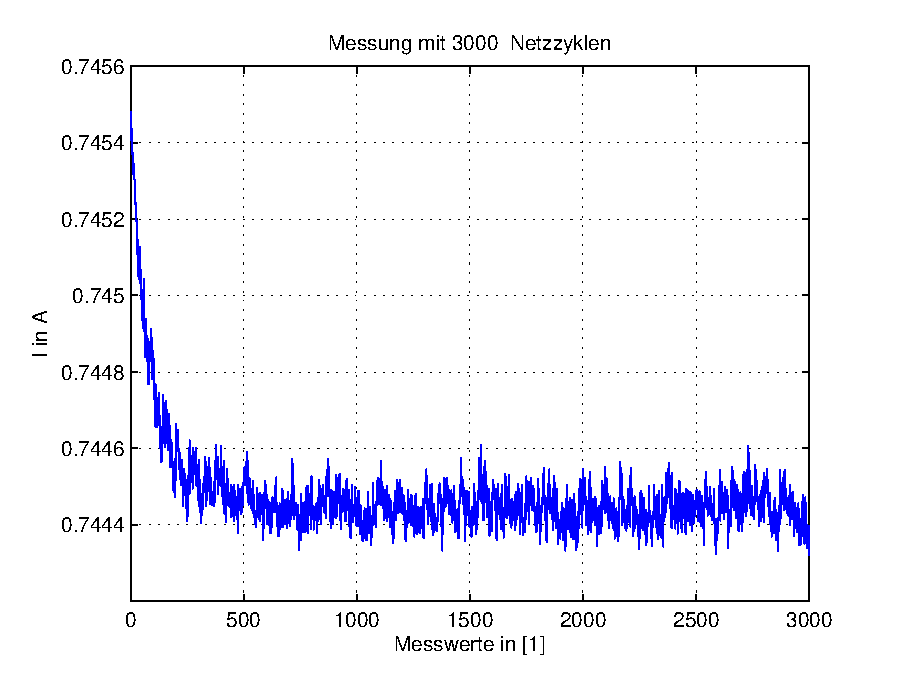
\includegraphics[scale=0.60]{./img/1b13000.eps}
    }
    \caption{Graph 1}
\end{center}
\end{figure}
\end{frame}

\begin{frame}
\frametitle{Aufgabe 1b}
\framesubtitle{1: Messungen}
\begin{figure}[H]
\begin{center}
    \fbox{
        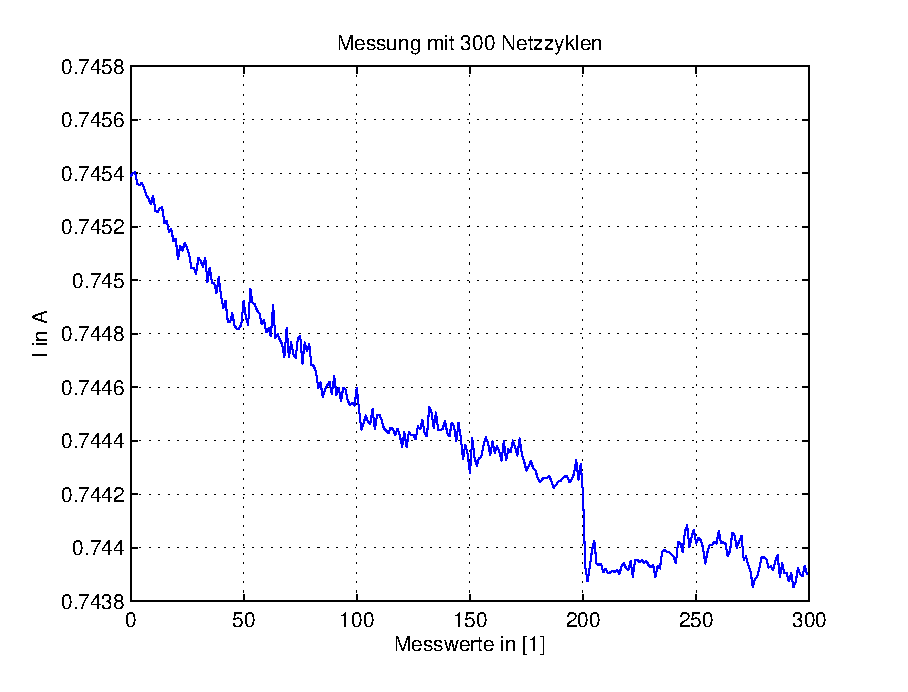
\includegraphics[scale=0.60]{./img/1b1300.eps}
    }
    \caption{Graph 2}
\end{center}
\end{figure}
\end{frame}
\begin{frame}
\frametitle{Aufgabe 1b}
\framesubtitle{Ergebnis}
    Man betrachtet:
    \begin{itemize}
        \item Starker Abfall der Stromstärke von $0-200$
        \item Annährung and den Endwert von $200-500$ in Graph $1$
        \item Sprung auf den Endwert bei $200$ in Graph $2$
    \end{itemize}
    Mögliche Erklärung:
     \begin{itemize}
         \item Bauteile des Geräts müssen sich erst aufwärmen oder einschwingen
         \item Bestimmte Bauteile funktionieren erst ab einer bestimmten
         Temperatur (Sprung in Graph $2$)
     \end{itemize}
    Sofortige Messung nach Einschalten des Geräts liefert keine verlässlichen
    Werte! \\
    Empfehlung des Herstellers: Gerät $30$ Minuten warmlaufen lassen
\end{frame}
\begin{frame}
\frametitle{Aufgabe 1b}
\begin{itemize}
    \item Die Wahl der Integrationszeit kann die Messung beeinflussen.
    \item Der Einfluss der Integrationszeit wurde durch verschiedene
    Netzzyklenzahlen und freie Zeiteinstellung getestet.
\end{itemize}
\end{frame}
\begin{frame}
\frametitle{Aufgabe 1b}
\framesubtitle{2:Messungen}
\begin{tabular}{c|c c c c}
    NPLC   & Maximum    & Minimum    & Mittelwert  &Standardabweichung \\
    \hline
    0,006  & 0,201529   & 0,19882    & 0,20011369  &5,69E-04\\
    0,02   & 0,201495   & 0,198794   & 0,200125373 &5,95E-04\\
    0,06   & 0,201637   & 0,198639   & 0,20012612  &7,70E-04\\
    0,2    & 0,201453   & 0,198895   & 0,200099427 &6,00E-04\\
    1      & 0,200122   & 0,200035   & 0,200076633 &1,54E-05\\
    10     & 0,20006    & 0,199953   & 0,199991067 &2,57E-05
\end{tabular}
\end{frame}
\begin{frame}
\frametitle{Aufgabe 1b}
\framesubtitle{2: Ergebnis}
     Je größer die Standardabweichung, desto mehr liegen Minima und Maxima
     voneinander entfernt $\rightarrow$ mehr Rauschen
     \begin{itemize}
         \item Größte Standardabweichung bei $0.6$ NPLC
         \item Kleinste Standardabweichung bei $10$ NPLC
     \end{itemize}
     $\rightarrow$ Beim Mitteln über Teilzyklen hebt sich das Rauschen nicht
     auf \\
     $\rightarrow$ Beim Mitteln über ganzzahlige Netzzyklen wird das Rauschen
     herausgefiltert \\
     $\rightarrow$ Erhöhung der ganzzahligen Netzzyklen verbessert die
     Genauigkeit
\end{frame}
\begin{frame}
\frametitle{Aufabe 1b}
\framesubtitle{3:Messungen}
\begin{tabular}{c|c c c c}
    NPLC   & Maximum    & Minimum    & Mittelwert  &Standardabweichung \\
    \hline
    0,006  & 0,201529   & 0,19882    & 0,20011369  &5,69E-04\\
    0,02   & 0,201495   & 0,198794   & 0,200125373 &5,95E-04\\
    0,06   & 0,201637   & 0,198639   & 0,20012612  &7,70E-04\\
    0,2    & 0,201453   & 0,198895   & 0,200099427 &6,00E-04\\
    1      & 0,200122   & 0,200035   & 0,200076633 &1,54E-05\\
    10     & 0,20006    & 0,199953   & 0,199991067 &2,57E-05\\
    \hline
    freie Int.& & & &\\
    \hline
    25 ms  & 0,200182   & 0,199796   & 0,19999138  &1,16E-04
\end{tabular}
\end{frame}
\begin{frame}
\frametitle{Aufgabe 1b}
\framesubtitle{3: Ergebnis} 
    Mitteln über eine frei gewählte Zeit ist ungenauer als vielfache NPLCs. \\
    $\rightarrow$ Netzzyklen werden nicht exakt abgeschlossen, Rauschen wird
    nicht vollständig weggehoben

    Wie soll gemittelt werden?
    \begin{itemize}
        \item Teilzyklen: erhöht Rauschen aber verkürzt Messzeit $\rightarrow$
        nur bei sehr vielen Messreihen
        \item vielfache NPCLs: verringert Rauschen aber längere Messzeit
        \item freie Zeit: Nur wenn freie Integrationszeit notwendig
    \end{itemize}
\end{frame}



\section{Invertierender Verstärker} % (fold)
\label{sec:Invertierender_Verstärker}
% section Invertierender Verstärker (end)

\section{Sequentielle Logik} % (fold)
\label{sec:Sequentielle Logik}
\subsection{RS-Flipflop} % (fold)
\label{sub:RS-Flipflop}
\begin{frame}
    \frametitle{RS-Flipflop}
    \framesubtitle{}
    \begin{figure}[H]
    \begin{center}
            \includegraphics[scale=0.5]{./img/schaltung/RS-FF.png}
    \end{center}
    \end{figure}
\end{frame}
\begin{frame}
    \frametitle{Funktionsweise}
    \framesubtitle{}
    \begin{columns}[c]
        \column{0.6\textwidth}
            \boxed{
                \begin{tabular}{c|c||c}
                    $\bar{S}$ & $\bar{R}$ & Q \\
                    \hline
                    1 & 1 & unverändert \\
                    0 & 1 & 1 (gesetzt) \\
                    1 & 0 & 0 (zurückgesetzt) \\
                    0 & 0 & Glitch ($Q = \bar{Q}$)
                \end{tabular}
                }
            \begin{block}{Gleizeitiges Auslößen}
                \begin{itemize}
                    \item ????
                \end{itemize}
            \end{block}
        \column{0.4\textwidth}
            \begin{figure}[H]
            \begin{center}
                    \includegraphics[scale=0.5]{./img/schaltung/RS-FF.png}
            \end{center}
            \end{figure}
    \end{columns}
\end{frame}
% subsection RS-Flipflop (end)

\subsection{Taktgesteuertes RS-Flip-Flop} % (fold)
\label{sub:Taktgesteuertes RS-Flip-Flop}
\begin{frame}
    \frametitle{Taktgesteuertes RS-Flip-Flop}
    \framesubtitle{}
     \begin{figure}[H]
     \begin{center}
             \includegraphics[scale=0.6]{./img/schaltung/RS-FF-T.png}
     \end{center}
     \end{figure}
\end{frame}
\begin{frame}
    \frametitle{Funktionsweise}
    \framesubtitle{}
    \begin{columns}[c]
        \column{0.6\textwidth}
            \boxed{
                \begin{tabular}{c|c|c||c}
                    S & R & C & Q \\
                    \hline
                     0 & 0 & 0 & unverändert \\
                     0 & 1 & 0 & unverändert \\
                     1 & 0 & 0 & unverändert \\
                     1 & 1 & 0 & unverändert \\
                     \hline
                     0 & 0 & 1 & unverändert \\
                     0 & 1 & 1 & 0 (zurückgesetzt) \\
                     1 & 0 & 1 & 1 (gesetzt) \\
                     1 & 1 & 1 & Glitch ($\bar{Q} = Q$)
                \end{tabular}
            }
        \column{0.4\textwidth}
             \begin{figure}[H]
             \begin{center}
                     \includegraphics[scale=0.6]{./img/schaltung/RS-FF-T.png}
             \end{center}
             \end{figure}
             \begin{figure}[H]
             \begin{center}
                     \includegraphics[scale=0.32]{./img/Aufgabe_2_b.eps}
             \end{center}
             \end{figure}
    \end{columns}
\end{frame}
% subsection Taktgesteuertes RS-Flip-Flop (end)

\subsection{D-Latch} % (fold)
\label{sub:D-Latch}
\begin{frame}
    \frametitle{D-Latch}
    \framesubtitle{}
    \begin{figure}[H]
    \begin{center}
            \includegraphics[scale=0.6]{./img/schaltung/D-Latch.png}
    \end{center}
    \end{figure}
\end{frame}
\begin{frame}
    \frametitle{Funktionsweise}
    \framesubtitle{}
    \begin{columns}[c]
        \column{0.6\textwidth}
            bla 
        \column{0.4\textwidth}
            \begin{figure}[H]
            \begin{center}
                    \includegraphics[scale=0.6]{./img/schaltung/D-Latch.png}
            \end{center}
            \end{figure}
            \begin{figure}[H]
            \begin{center}
                    \includegraphics[scale=0.3]{./img/Aufgabe_2_c.eps}
            \end{center}
            \end{figure}
    \end{columns}
\end{frame}
% subsection D-Latch (end)

\subsection{Flankengetriggertes D-Latch} % (fold)
\label{sub:Flankengetriggertes D-Latch}
\begin{frame}
    \frametitle{Flankengetriggertes D-Latch}
    \framesubtitle{}
     \begin{figure}[H]
     \begin{center}
             \includegraphics[scale=0.3]{./img/schaltung/flanken_d.png}
     \end{center}
     \end{figure}
\end{frame}
\begin{frame}
    \frametitle{Flankengetriggertes D-Latch}
    \framesubtitle{}
     \begin{columns}[c]
         \column{0.6\textwidth}
         \begin{figure}[H]
         \begin{center}
                 \includegraphics[scale=0.25]{./img/schaltung/flanken_d.png}
         \end{center}
         \end{figure}
         \column{0.4\textwidth}
         \begin{figure}[H]
         \begin{center}
                 \includegraphics[scale=0.3]{./img/Aufgabe_3_d.eps}
         \end{center}
         \end{figure}
     \end{columns}
     \begin{block}{Funktionsweise}
        \begin{itemize}
            \item Clock muss vor Triggerung auf 1 stehen 
            \item Flanken werden nicht erkannt
        \end{itemize}
     \end{block}
\end{frame}
% subsection Flankengetriggertes D-Latch (end)

% section Sequentielle Logik (end)

\section{Zähler} % (fold)
\label{sec:Zähler}
\begin{frame}
    \frametitle{Zähler}
    \framesubtitle{}
     \begin{figure}[H]
     \begin{center}
             \includegraphics[scale=0.3]{./img/schaltung/zahler.png}
     \end{center}
     \end{figure}
\end{frame}
\begin{frame}
    \frametitle{Entwicklung}
    \framesubtitle{}
    \begin{columns}[c]
        \column{0.5\textwidth}
         \begin{block}{Funktionsweise}
            \begin{itemize}
                \item D-Latch flipt aktuelles Bit 
                \item falls Q gesetzt wird $\bar{Q}$ und somit der nächste D-Latch
                gesetzt
                \item Zahl muss 'rückwärts' gelesen werden
            \end{itemize}
         \end{block}
        \column{0.5\textwidth}
             \begin{center}
                \boxed{
                    \begin{tabular}{c}
                        0000 \\
                        1000 \\
                        0100 \\
                        1100 \\
                        0010 \\
                        1010 \\
                        1110 \\
                        0001 \\
                        1001 \\
                        0101 \\
                        1101 \\
                        0011 \\
                        1011 \\
                        0111 \\
                        1111 \\
                    \end{tabular}
                }
             \end{center}
    \end{columns}
\end{frame}
% section Zähler (end)

\begin{frame}
\frametitle{Aufgabe 5a}
\framesubtitle{}
\begin{itemize}
    \item Mit Labview wurden Störfrequenzen in das Signal eingespeist
    \item Analyse der störenden Frequenzen im Oszilloskop
\end{itemize}
Gemessene Störfrequenzen:
\begin{center}
    \begin{tabular}{c|c}
        Gerät & Frequenz/kHz \\
        \hline
        PC & 53.7 \\
        Monitor & 55.0, 66.5 \\
        Oszillosop & 57.3 \\
        DMM & 94.1 \\
        Frequenzgenerator &45.6,60.6 \\
        Kaffeemaschine & keine erkennbaren Frequenzen
    \end{tabular}
\end{center}
\end{frame}

\begin{frame}
\frametitle{Aufgabe 5b}
\framesubtitle{}
    \begin{itemize}
        \item Messung der Störung kleiner Spannungen durch Versuchsgeräte.
        \item Wiederholte Messung bei nähergelegten Kabeln
    \end{itemize}
\end{frame}
\begin{frame}
\frametitle{Aufgabe 5b}
\framesubtitle{}
\begin{center}
    \begin{tabular}{c|c}
        Gerät & Frequenz/kHz \\
        \hline
        Funktionsgenerator & 44.4 , 57,1, 62.3, 82,4, 76.0 \\
        DMM & 57.1 , 81.1 \\
        Monitor& 47.7 , 55.8, 64.2
    \end{tabular}

Mit Koaxialkabel: Keine Störungen. \\
$\rightarrow$  Der räumliche Versuchsaufbau hat Auswirkung auf die Messung \\
$\rightarrow$  Zur exakter Messung Störquellen vom Messort entfernen, oder
Koaxialkabel verwenden \\
$\rightarrow$ Keine unnötigen Geräte betreieben
\end{center}
\end{frame}

    
\end{document}
